% !TEX encoding = UTF-8 Unicode
\documentclass[pdftex, a4paper,12pt]{article}

\usepackage[utf8]{inputenc}
\usepackage[T1]{fontenc}
\usepackage[french]{babel}
\usepackage[pdftex]{graphicx}
\usepackage{xcolor}
\usepackage{listingsutf8}
\usepackage{geometry}

\geometry{left=2cm, right=2cm, top=2cm, bottom=2cm}
\newcommand{\HRule}{\rule{\linewidth}{0.5mm}} 

\lstset{
	frame=tb,
	captionpos=b,
	inputencoding=utf8/latin1,
	breaklines=true,
	showstringspaces=true,
	columns=flexible,
	tabsize=4,
	breakatwhitespace=true
}
\begin{document} 

\begin{titlepage}
%\geometry{left=2cm, right=2cm, top=2cm, bottom=2cm}
\begin{center}


\includegraphics[width=0.15\textwidth]{./Logo_INSA_RN}\\[1cm]    

\textsc{\Large PROJET D'APPROFONDISSEMENT ET D'OUVERTURE}\\[0.5cm]

\HRule \\[0.8cm]
{\LARGE \bfseries COMPAGNON VIRTUEL SOUS ANDROID}\\[0.4cm]

\HRule \\[1.5cm]

\textsc{Institut national des sciences appliquées de Rouen}\\[1.5cm]

% Author and supervisor
\begin{minipage}{0.4\textwidth}
\begin{flushleft} \large
\emph{Rédigé par:}\\
Jitao \textsc{XU}

Chenxin \textsc{LU}
\end{flushleft}
\end{minipage}
\begin{minipage}{0.4\textwidth}
\begin{flushright} \large
\emph{Proposé par:} \\
Alexandre \textsc{PAUCHET}
\end{flushright}
\end{minipage}

\vfill

% Bottom of the page
\textsc{\large ASI}\\
{\large \today}

\end{center}
\end{titlepage}

\tableofcontents

\addcontentsline{toc}{section}{Introduction}
\newpage

\section*{Introduction}


Dans le cadre de notre scolarité au sein du département Architecture des Systèmes d’Information (ASI) de l’Institut National des Sciences Appliquées (INSA) de Rouen, nous devons réaliser au cours de notre premier semestre de quatrième année un Projet d’Approfondissement et d’Ouverture (PAO), c’est-à-dire un travail sur plusieurs mois, seul ou en équipe, dans lequel nous pouvons mettre en pratique nos connaissances apprises en cours et/ou apprendre de nouvelles connaissances sur des sujets en rapport avec notre formation.
Nous avons donc tous les deux décidé de nous intéresser à un sujet proposé par M. Alexandre Pauchet : la création d’un compagnon virtuel sous Android. Ce PAO permet d’une part de mettre en application nos acquis en Java de troisième année, et d’autre part de découvrir la conception d’une application mobile sous Android, chose totalement nouvelle pour nous deux.


\pagenumbering{arabic}
\newpage
\section*{Chapitre1}
\section{Analsye des besoins}
\subsection{Liste des besoins}
Le but principal du projet est de développer des nouvelles fonctionnalités sur l'application Compagnon Virtuel déjà existante, notre verision sera version 4.
Avant de commencer le projet, l'application est déjà fonctionnelle, elle propose une interaction avec un personnage animé. Ce dernier est capable d'échanger via reconnaissance vocale et synthèse vocale. L'analyse des requêtes est déportée sur un serveur externe de dialogue intelligent: pandorabots. Le compagnon virtuel s'exprime aussi via des animations. Pendant la préparation du projet, nous avons proposé de réaliser les fonctionnalités suivantes:\\
	\indent- effectuer une recherche dans googlemaps et afficher une carte dans l'application.\\
	\indent- envoyer sms.\\
	\indent- ajouter et supprimer un réveil.\\
	\indent- afficher un calendrier au sein de l'application\\
	\indent- intégrer le processus de gestion de calendrier au chatbot externe.\\
	\indent- afficher le prochain événement dans le calendrier, il est capable de mettre à jour le prochain événement s'il y a une modification dans le calendrier.\\
	
Autrement, nous avons proposé de améliorer l'interface d'utilisateurs de l'application car nous n'étions pas satisfaits avec l'interface d'utilisateur actuelle.

\subsection{Rendus}
En résumé, les rendus demandés sont:\\
    \indent- une application fonctionnelle sous Android,\\
    \indent- un rapport sur le déroulement du projet,\\
    \indent- une documentation du code source,\\
    \indent- un guide utilisateur,\\
	\indent- une vidéo pour faire une démonstration d'application.\\
\indent Ils doivent être fournis avant la fin du premier semestre de ASI 4.1, afin d'être compabilisés dans la moyenne semestrielle.
\newpage

\section*{Chapitre 2}
\section{Spécification}
\subsection{Faisabilité du projet}
Dans un premier temps, nous avons suivi un cours sur www.udacity.com pour apprendre la base des connaissances de développer une application sous Android. Ce cours nous permet de développer une simple application, par exemple un compteur de points qui est utilisé dans le match du basket sous Android nous-même. Donc, nous pensons que nous sommes capable de commencer notre PAO.\\\\
\indent Ensuite, nous avons effectué une brève étude bibliographique quant à la faisabilité du développent de fonctionnalités que nous avons proposé. Nous avons trouvé des APIs du développement sous Android. Dans ce cas là, nous pensions que tous les fonctionnalités pouvaient être développés sous Android sans trop de difficulté. \\\\
\indent Concernant la partie de la réponse intelligente, comme les anciens PAOs sur ce sujet, nous avons décidé d'utiliser le Pandorabots, outils Internet permettant d'héberger un grand nombre de fichiers AIML contenant les question/réponses, pour nous aider de réaliser tous les fonctionnalités.
Le choix du IDE a été fait rapidement, nous avons choisi Android Studio qui est un IDE très moderne. \\\\
\indent Notre application peut être fonctionnée sur Android 4.4 ou supérieur avec une connexion Internet permanante.\\

\subsection{Analyse Descendante}
\begin{figure}[h]
\centering
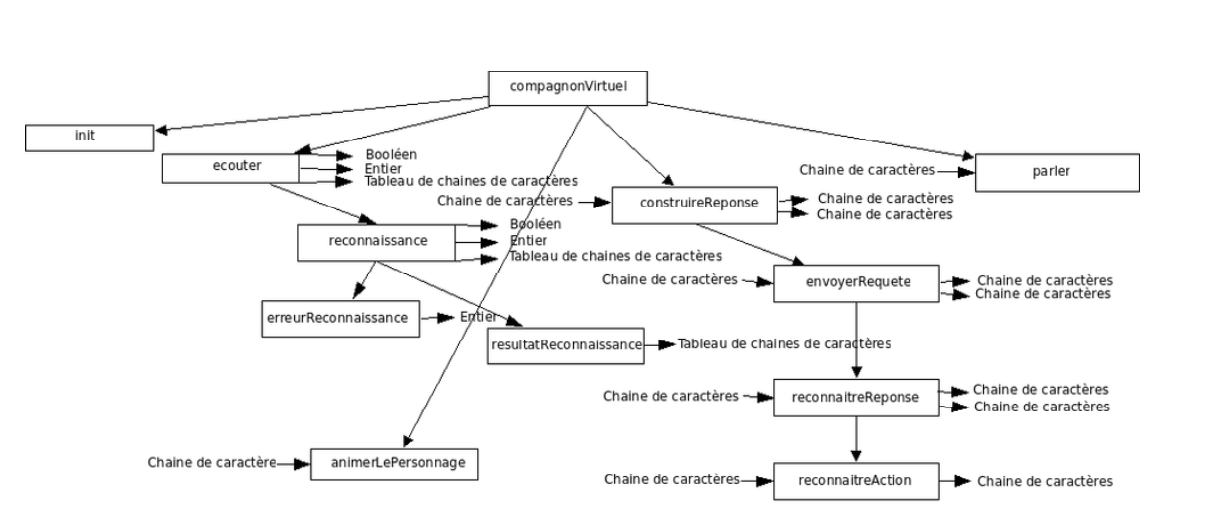
\includegraphics[width=1\linewidth]{analyseDescendante.png}
\caption{Analyse descendante de la version ancienne.\label{fig1}}
\end{figure}
\indent L'analyse descendante a été décrit dans le rapport  de 1ère version.
\newpage

\section*{Chapitre 3}
\section{Conception Préliminaire}
\indent Cette étape nous permet, à partir des différents éléments de l'analyse, de mettre en forme les fonctions et procédures afin d'en expliciter les nouveaux fonctionnements.

\subsection{Diagramme de cas d'utilisation}
\begin{figure}[ht]
\centering
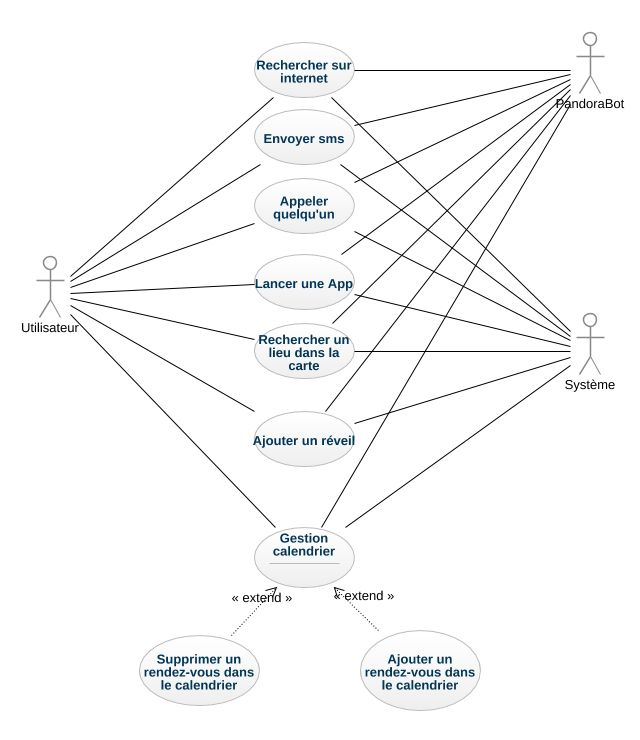
\includegraphics[scale=0.5]{./diagrammes/UsecaseDiagram.jpeg}
\caption{Diagramme de cas d'utilisation.\label{fig2}}
\end{figure}

\subsection{Diagramme de Sequence}
\begin{figure}[ht]
\centering
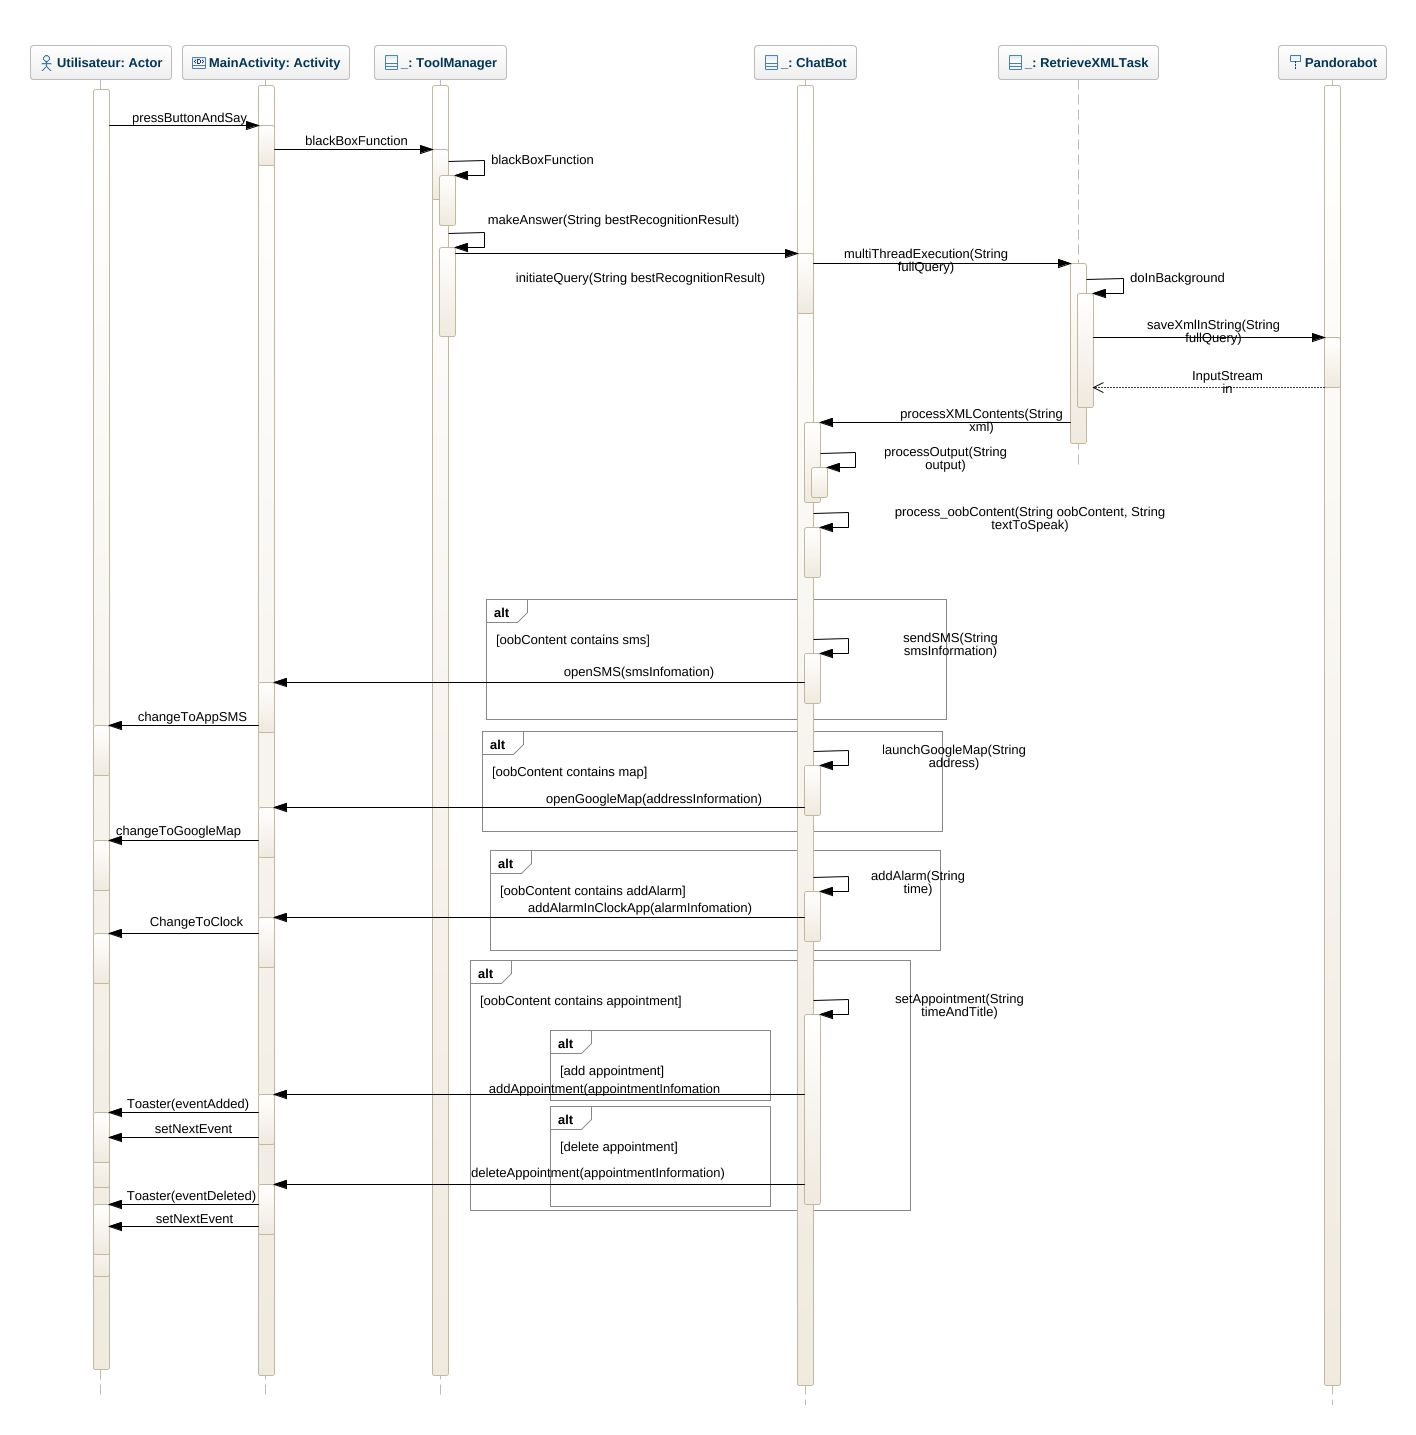
\includegraphics[scale=0.4]{./diagrammes/SequenceDiagram.jpeg}
\caption{Diagramme de Sequence.\label{fig3}}
\end{figure}
\indent La FIGURE \ref{fig3} représente un diagramme de séquence pour les fonctionnalités que nous avons proposé de réaliser. Les parties <<boite noire>> sont les parties du code qui ont été complétées dans les dernières versions. Ce que nous avons construit est la partie au-dessous de \textbf{\emph{process$_-$oobContent(String oobContent, String textToSpeak)}}.
\newpage

\subsection{Signatures Partie Chatbot}
procédure setAppointement (E/S Gcal : GestionCalendar, E oobContent : String, operationType : String)\\
\indent fonction setBeginTimeAndGetTitle (E oobContent : String, beginTime : Calendar, operationType : String) : String\\
\indent procédure googleQuery (E/S googleSearchText : String)\\
\indent procédure launchApp (E app : String)\\
\indent procédure launchUrl (E/S url : String)\\
\indent procédure launchGoogleMap (E/S address : String)\\
\indent procédure sendSMS (E oobContent : String)\\
\indent procédure makePhoneCall (E oobContent : String)\\
\indent procédure addAnAlarm(E oobContent : String)\\
\indent procédure deleteAnAlarm (E oobContent : String)\\

\subsection{Signatures Partie ToolManager}
procédure setNextEvent()\\
\indent fonction getNextEvent() : String\\
\newpage


\section*{Chapitre 3}
\section{Conception Détaillée}
\indent Cette étape nous permet, à partir de conception préliminaire, de préciser l'algorithme des fonctions ou procédures principales.

\subsection{addAnAlarme}
	\lstinputlisting[caption=addAnAlarm]{addAnAlarm}

\subsection{sendSMS}
	\lstinputlisting[caption=sendSMS]{sendSMS}

\subsection{setAppointement}
	\lstinputlisting[caption=setAppointement]{setAppointement}

\subsection{setBeginTimeAndGetTitle}
	\lstinputlisting[caption=setBeginTimeAndGetTitle]{setBeginTimeAndGetTitle}
	
\subsection{getNextEvent}
	\lstinputlisting[caption=getNextEvent]{getNextEvent}
\section*{Chapitre 5}
\section{Développememnt}
	La partie développement s'est déroulée en quatre sous parties. Tout d'abord, nous nous sommes informés des méthodes proposées sur Android pour mettre en place les fonctionnalités précisés dans le Chapitre 4. Ensuite nous avons ajouté plusieurs catégories de questions/réponses sur le site Pandorabots pour faire fonctionner nos fonctionnalités. Enfin, nous avons modifié l'interface d'utilisateurs de l'application pour améliorer l'expérience d'utilisation. Dans ce cas là, Nous avons changé le personnage d'animation pour afficher plus d'informations sur l'activité principale. Ces quatre sous parties ont été implémenté itérativement tout au long du développement.

\subsection{Mis en place des différentes foncitonnalités}
	
\indent Comme nous l'avons dit précédemment, nous avons suivi un cours sur \emph{www.udacity.com} pour apprendre la base de développer une application sous Android et nous avons effectué une recherche bibliographique pour mettre en place les foncition suivantes : launchGoogleMap, sendSMS, addAnAlarm, deleteAnAlarm, setAppointement, getNextEvent, setNextEvent. Les cinq premières fonctions ont été implémenté dans la classe Chatbot, les deux suivantes dans la classe ToolManager.\\
\indent Toutes les foncitions sont appelées dans la méthode \textbf{\emph{process$_-$oobContent(String oobContent, String textToSpeak)}} sauf getNextEvent et setNextEvent. Le paramètre oobContent contient l'information retourner par le serveur Pandorabots entre "<oob>" et "</oob>". Le deuxième "textToSpeak" ne concerne pas nos fonctions.

\subsubsection{Lancer Google Map}

\indent Premièrement, selon notre recherche, toutes les chaînes de caractère transmises aux intentions Google Maps doivent être encodées sous forme d'URI. Dans notre fonction, il faut remplacer tous les espaces ' ' par "\%20" ou '+'. Nous avons choisi de les remplacer par '+'. Ensuite, nous avons créé un instance de \textbf{\emph{Intent}}, qui permet de lancer une application depuis l'activité actuelle. 

\indent En effet, nous avions essayé d'afficher la carte de Google Map dans notre application, néanmoins elle ne garde pas tous les fonctionnalité de l'application Google Map. Nous avons donc décidé de l'abandonner. Nous allons le préciser dans la chapitre 6.

\subsubsection{Envoyer SMS}
\indent Nous proposons deux types de destination du sms : un numéro de téléphone mobile ou un correspondant dans le carnet d'adresses.  Pour les réaliser, il faut toujours déterminer le type de première caractère de destination. Si c'est une lettre, donc nous prenons le mode 'correspondant', sinon, nous prenons le mode 'numéro de téléphone mobile'. Grâce au instance \textbf{\emph{Intent}}, notre fonction pouvons lire le String qui décrit la destination du sms. 

\indent Si nous sommes tombé dans le deuxième mode, nous allons chercher le numéro de téléphone mobile dans le carnet d'adresses, et puis envoyer le sms par le numéro.\\

\indent Pareil, nous écrivons le contenu du sms par l'instance \textbf{\emph{Intent}}.
	
\subsubsection{Ajouter et Supprimer un réveil}
\indent Idée principale :

\indent Pour ajouter un réveil, simplement, nous déterminons la date et l'heure du réveil avec la reconnaissance vocale. Ensuite, nous utilisons toujours un instance de \textbf{\emph{Intent}} qui nous permet de réaliser l'ajout des informations pour un réveil. Après, c'est important de déterminer la répétition du réveil. Par différents chaines de caractères, nous trouvrons la demande de répétition d'utilisateur. Finalement, nous finisons l'ajout du réveil.

\indent Pour supprimer un réveil, c'est plus simple. Nous cherchons la date et l'heure du réveil et le supprimer directement.

\indent Pour les détails du code: 

\indent Nous avons trouvé que la chaîne de reconnaissance vocale pour le temps est sous format "*h*", par exemple "14h35". Nous avons donc séparé la chaîne par 'h' et pris la première partie comme l'heure du réveil. Nous avons mis la minute du réveil à 0 par défaut s'il manque la deuxième partie dans la chaîne. Il faut ajouter une permission de régler l'alarme dans le fichier \textbf{\emph{AndroidManifest.xml}} : \\
	\begin{lstlisting}[frame=none,aboveskip=-0.5em,basicstyle=\footnotesize\bfseries]
	<uses-permission android:name="com.android.alarm.permission.SET_ALARM"/>
	\end{lstlisting}

\indent Nous avons implémenté la fonction \textbf{\emph{deleteAnAlarm(String oobContent)}}. Pour réaliser la fonctionnalité, nous devions utiliser une constante \textbf{\emph{AlarmClock.ACTION$_-$DISMISS$_-$ALARM}} qui a besoin d'une API au niveau supérieur ou égal à 23. Cependant, les appareils que nous avions ne possédait qu'au niveau 19. En conséquence, nous ne pourrions pas réaliser cette fonctionnalité.Nous allons le préciser dans la chapitre 6.

\subsubsection{Gestion du rendez-vous}
\subsubsection*{Ajouter et Supprimer un rendez-vous}

\indent Nous avons modifié la version précédente pour intégrer le traitement de gestion de calendrier au serveur externe, Pandorabots. Nous avons gardé les méthodes pour initialiser l'instance de \textbf{\emph{GestionCalendar}} et les méthodes \textbf{\emph{ajouterRDV(String titre, Calendar beginTime, Calendar endTime)}} et \textbf{\emph{supprimerRDV(String titre, Calendar beginDate,Calendar endDate)}}. Ces deux dernières nous permet d'ajouter ou de supprimer un rendez-vous dans l'agenda de l'appareil.

\indent Nous avons créer une méthode \textbf{\emph{setAppointement(GestionCalendar Gcal, String oobContent, String operationType)}} qui nous permet de distinguer l'ajout et la suppression du rendez-vous. Pour pouvoir utiliser les méthodes déjà existantes, il faut avoir le titre, la date de début et la date de fin du rendez-vous. Pour simplifier le traitement, nous avons créer une méthode \textbf{\emph{setBeginTimeAndGetTitle(String oobContent, Calendar beginTime, String operationType)}} qui régler la date de début et retourner le titre de rendez-vous en même temps. Dans cette dernière méthode, le paramètre \textbf{\emph{beginTime}} en entrée est la date actuel du système. Nous avons met à défaut toutes les parties de la date commes la date actuel. Nous avons vérifié la chaîne \textbf{\emph{oobContent}} dans l'ordre suivantes : jour, mois, an, heure, minute, titre. Pour chaque partie précisée, nous avons met à jour l'information. Si l'utilisateur n'a pas précisé le titre du rendez-vous, le titre par défaut sera une chaîne vide.

\indent La méthode \textbf{\emph{setBeginTimeAndGetTitle}} permet l'utilisateur de ne pas préciser n'importe quelle partie d'une date tant que les informations précisées sont dans l'ordre.

\subsubsection*{Mettre à jour le prochain rendez-vous}

\indent Nous avons aussi supprimé la méthode \textbf{\emph{prochainRDV}} pour créer une nouvelle dans la classe \textbf{\emph{ToolManager}}. La méthode \textbf{\emph{getNextEvent()}} permet de retourner une chaîne de caractère qui contient les informations du prochain rendez-vous. Dans la méthode, nous avons créer un instance de \textbf{\emph{Cursor}} qui peut se déplacer comme un pointeur. Nous cherchions dans la liste d'événement stocké dans l'agenda de l'appareil pour trouver l'événement le plus proche de la date actuel.

\subsection{Ajout plusieurs catégories de questions/réponses sur le site Pandorabots}

\indent Nous continuions à utiliser le compte créé par les étudiants précédents pour ajouter des catégories de questions/réponses sur \textbf{\emph{https://www.pandorabots.com/botmaster/fr/home}}, avec les identifiants suivants:

\begin{center}
	Email : \textbf{\emph{alexandre.levacher@insa-rouen.fr}}\\
	Mot de passe : \textbf{\emph{PAOCompagnonVirtuel3}}
\end{center}

\indent Tout les informations d'une quesion/réponse sont comprises entre \textbf{\emph{<category>}} et \textbf{\emph{</cagegory>}}. La balise \textbf{\emph{<pattern>}} contient la question et la balise \textbf{\emph{<template>}} est la partie de réponse intelligente. La balise \textbf{\emph{<oob>}} se situe dans la balise \textbf{\emph{<template>}}.

\subsubsection{Ajouter un réveil sans répétition}
\begin{lstlisting}[frame=none,aboveskip=0.5em]
<category><pattern>SONNER POUR *</pattern><template><oob><alarmclock>
<add><star/></add></alarmclock></oob></template></category>
\end{lstlisting}

\begin{lstlisting}[frame=none,aboveskip=0.5em]
<category><pattern>AJOUTER UN RÉVEIL À * </pattern><template><srai>SONNER POUR <star/></srai></template></category>
\end{lstlisting}

\begin{lstlisting}[frame=none,aboveskip=0.5em]
<category><pattern>AJOUTER UN RÉVEIL POUR * </pattern><template><srai>SONNER POUR <star/></srai></template></category>
\end{lstlisting}

\subsubsection{Ajouter un réveil avec répétition}
\begin{lstlisting}[frame=none,aboveskip=0.5em]
<category><pattern>AJOUTER UN RÉVEIL À * POUR TOUS LES * </pattern><template><oob><alarmclock><add><star index="1"/></add><repetition><star index="2"/></repetition></alarmclock></oob></template></category>
\end{lstlisting}

\begin{lstlisting}[frame=none,aboveskip=0.5em]
<category><pattern>AJOUTER UN RÉVEIL POUR * POUR TOUS LES * </pattern><template><srai>AJOUTER UN RÉVEIL À<star index="1"/>POUR TOUS LES<star index="2"/></srai></template></category>
\end{lstlisting}

\begin{lstlisting}[frame=none,aboveskip=0.5em]
<category><pattern>AJOUTER UN RÉVEIL POUR TOUS LES * POUR * </pattern><template><srai>AJOUTER UN RÉVEIL À<star index="2"/>POUR TOUS LES<star index="1"/></srai></template></category>
\end{lstlisting}

\begin{lstlisting}[frame=none,aboveskip=0.5em]
<category><pattern>AJOUTER UN RÉVEIL POUR TOUS LES * À * </pattern><template><srai>AJOUTER UN RÉVEIL À<star index="2"/>POUR TOUS LES<star index="1"/></srai></template></category>
\end{lstlisting}

\subsubsection{Supprimer un réveil}
\begin{lstlisting}[frame=none,aboveskip=0.5em]
<category><pattern>SUPPRIMER UN RÉVEIL DE *</pattern><template><oob>
<alarmclock><delete><star/></delete></alarmclock></oob></template></category>
\end{lstlisting}

\begin{lstlisting}[frame=none,aboveskip=0.5em]
<category><pattern>SUPPRIMER UN RÉVEIL À *</pattern><template><srai>SUPPRIMER UN RÉVEIL DE <star/></srai></template></category>
\end{lstlisting}

\subsubsection{Ajouter un rendez-vous}
\begin{lstlisting}[frame=none,aboveskip=0.5em]
<category><pattern>AJOUTER UN RENDEZ-VOUS LE *</pattern><template><oob><appointment><add><eventdate><star/></eventdate></add></appointment></oob></template></category>
\end{lstlisting}

\begin{lstlisting}[frame=none,aboveskip=0.5em]
<category><pattern>AJOUTER UN RENDEZ-VOUS LE * À * , *</pattern><template><oob><appointment><add><eventdate><star index="1"/></eventdate><eventtime><star index="2"/></eventtime><event><star index="3"/></event></add></appointment></oob></template></category>
\end{lstlisting}

\begin{lstlisting}[frame=none,aboveskip=0.5em]
<category><pattern>AJOUTER UN RENDEZ-VOUS LE * À *</pattern><template><oob><appointment><add><eventdate><star index="1"/></eventdate><eventtime><star index="2"/></eventtime></add></appointment></oob></template></category>
\end{lstlisting}

\subsubsection{Supprimer un rendez-vous}
\begin{lstlisting}[frame=none,aboveskip=0.5em]
<category><pattern>SUPPRIMER UN RENDEZ-VOUS LE *</pattern><template><oob><appointment><delete><eventdate><star/></eventdate></delete></appointment></oob></template></category>
\end{lstlisting}

\begin{lstlisting}[frame=none,aboveskip=0.5em]
<category><pattern>SUPPRIMER UN RENDEZ-VOUS LE * À * INTITULÉ *</pattern><template><oob><appointment><delete><eventdate><star index="1"/></eventdate><eventtime><star index="2"/></eventtime><event><star index="3"/></event></delete></appointment></oob></template></category>
\end{lstlisting}

\begin{lstlisting}[frame=none,aboveskip=0.5em]
<category><pattern>SUPPRIMER UN RENDEZ-VOUS LE * INTITULÉ *</pattern><template><oob><appointment><delete><eventdate><star index="1"/></eventdate><eventtime>0</eventtime><event><star index="2"/></event></delete></appointment></oob></template></category>
\end{lstlisting}

\subsubsection{Réaliser une recherche en Google Map}
\begin{lstlisting}[frame=none,aboveskip=0.5em]
<category><pattern>_MAPS *</pattern><template><oob><maps><star/></maps></oob></template></category>
\end{lstlisting}

\begin{lstlisting}[frame=none,aboveskip=0.5em]
<category><pattern>_ MAPS *</pattern><template><oob><maps><star/></maps></oob></template></category>
\end{lstlisting}

\subsubsection{Envoyer un sms}
\begin{lstlisting}[frame=none,aboveskip=0.5em]
<category><pattern>_ENVOYER UN SMS POUR * POUR DIRE *</pattern><template><oob><send><people><star index="1"/></people><message><star index="2"/></message></send></oob></template></category>
\end{lstlisting}

\begin{lstlisting}[frame=none,aboveskip=0.5em,belowskip=1.5em]
<category><pattern>_ENVOIE UN SMS POUR * POUR DIRE *</pattern><template><oob><send><people><star index="1"/></people><message><star index="2"/></message></send></oob></template></category>
\end{lstlisting}



\subsection{Modification de l'interface d'utilisateur}
\indent Premièrement, nous avons séparé le centre de l'interface d'utilisateur à deux partie. La partie gauche affiche les cinq reconnaissaces vocales du voix de l'utilisateur plus possibles. La partie droite affiche la réponse de notre application s'il existe. En bas de l'écran, nous avons ajouté un \textbf{\emph{textField}} pour afficher le prochain événement dans le calendrier. Ce \textbf{\emph{textField}} va se mettre à jour s'il existe un changement d'événement plus proche dans le calendrier grâce à la fonction \textbf{\emph{getNextEvent}}. Autrement, nous avons changé le personnage d'animation. Nous allons parler dans la paragraphe suivante.

\subsection{Changement du personnage}
\indent Nous avons choisi un personnage d'animation de Microsoft qui est open source. Nous avons téléchargé l'ensemble d'image du personnage tout d'abord. Puis, nous avons utilisé l'outil pour le couper par chaque action. Pour différentes actions, nous avons proposé un temp de continu. Avec ces images, nous avons réalisé les animations  suivantes: saluer, écouter, trouver une  erreur, parler, rire, répondre, etc. Ce changement du personnage améliore notre l'interface d'utilisateur, de plus, il nous permet d'avoir plus d'espace sur l'écran pour afficher d'autres informations. Nous pensons que c'est un changement indispensable.

\newpage





\end{document}
